C{\sc \,iii}]$\,\lambda$1906\ang
O{\sc \,iii}]$\,\lambda\,1666$

Al{\sc \,iii}

Si{\sc ii}$\lambda\,$1260


We show that assuming a fixed relationship between [N/H] and [C/H] with [O/H] does not match observations, and derive a relationship for N and C enrichment that improves the performance of photoionization models. We also examine the effects of decoupling the stellar metallicity from the gas phase metallicity, which may be appropriate for high redshift galaxies where high SFRs may rapidly enrich the gas in $\alpha$-elements.


The line list was seeded from lists of observed emission lines and filled in with emission lines that were relatively strong in \Cloudy models over the full range in age, metallicity, and ionization parameter considered in this work.

%-------------------------------------------------------
% Absorption Indices
%-------------------------------------------------------
\begin{figure*}
  \begin{center}
    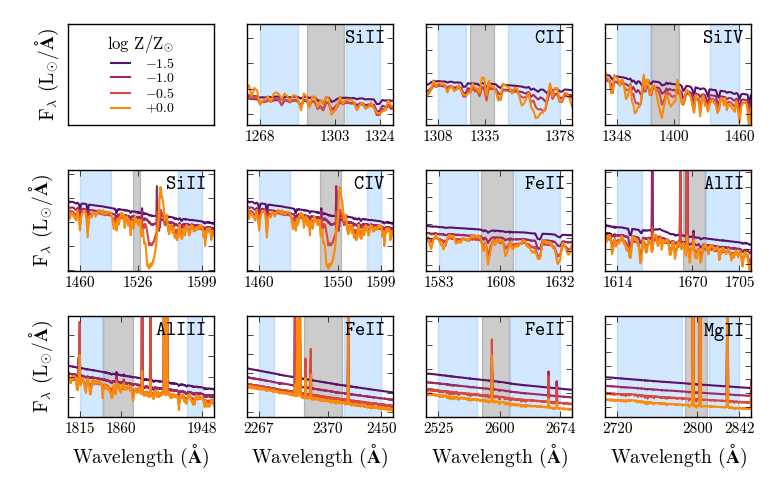
\includegraphics[width=0.95\linewidth]{figs/f3.png}
    \caption{We show the absorption indices defined by \citet{Leitherer+2011} for a stellar population with constant SFR at 10\Myr with \logUeq{-2.5} at \logZeq{-1.5}, $-1.0$, $-0.5$, and $+0.0$. Each panel shows a different index, noted in the top right corner. The shaded regions show the wavelength ranges of the red and blue continuum and the central bandpass used to measure the equivalent width of the feature. The line indices are a combination of stellar photospheric absorption lines, stellar wind lines, and blends of lines. We note that many of the defined bandpasses include nebular emission, which changes their utility as metallicity diagnostics.}
    \label{fig:lineIndex}
  \end{center}
\end{figure*} 
%-------------------------------------------------------

\section{Decoupled gas and stellar metallicities}\label{appdx:gasZ}

Our models assume that the massive stars that dominate the UV stellar continuum have the same metallicity and abundance pattern as the gas that they ionize. However, there are scenarios in which it is possible that the gas phase abundances differ from the stellar abundances. These include the injection of metal-enriched gas from stellar outflows or the rapid accretion of metal-poor gas during fueling of a star formation event. The latter of these would likely be most important during early epochs of star formation, with high gas inflow rates, which would be required for accretion to dilute the gas on $<10$\Myr timescales. Early star formation could also take place in gas enriched in $\alpha$-elements, due to the reduced fraction of Type Ia supernovae (SNe).

Recently, \citet{Steidel+2016} have suggested that the stellar and gas phase abundances should be decoupled due to the $\alpha$ enhancement of the gas relative to the stellar population. In their scenario, to first order, the stellar metallicity will follow the iron abundances while the gas metallicity should follow the measured oxygen abundances. From Salpeter IMF-averaged yields for O/Fe based on core collapse supernovae, \citet{Steidel+2016} estimates that this could produce nebular oxygen abundances that are 4-5 times larger than the stellar Fe-based metallicity. 

We have generated models where both the gas and stellar abundances are allowed to vary to explore the observable consequences of this choice.

We cannot self-consistently model $\alpha-$enhanced gas, since the MIST models used in this work for the stellar ionizing spectrum rely on solar-scaled abundances. To mimick the effects of $\alpha-$enhancement, we thus decouple the stellar metallicity from the gas phase metallicity and allow the relative gas phase abundances to increase above the stellar abundances. This will ``enhance'' the gas in $\alpha$-elements like O, Mg, Al, Ti, and Si, but will also enhance Fe-peak elements in the gas. We do not expect this to change the results qualitatively, since Fe does not play a large role in determining the thermodynamics of the gas. 

We first model the ``enriched gas'' scenario by pairing a low-metallicity SSP (\logZeq{-1}) with moderate metallicity gas (\logZeq{-0.5}). These values are motivated by \citet{Steidel+2016}, who found that abundance determinations sensitive to stellar photospheric line blanketing features gave a metallicity of \logZeq{-1} while nebular emission lines, primarily optical oxygen and nitrogen lines, gave a metallicity of \logZeq{-0.4}, or Z$_{\mathrm{gas}}$ = $4\,$Z$_{\mathrm{star}}$.

%-------------------------------------------------------
% diffZ BPT
%-------------------------------------------------------
\begin{figure*}
  \begin{center}
    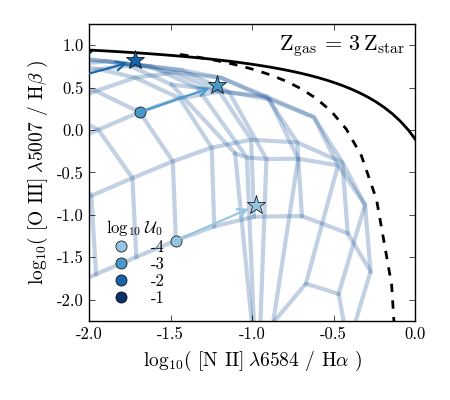
\includegraphics[width=0.283\linewidth]{figs/f27a.png}
    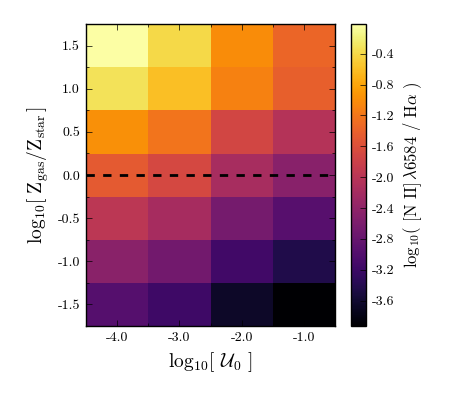
\includegraphics[width=0.283\linewidth]{figs/f27b.png}
    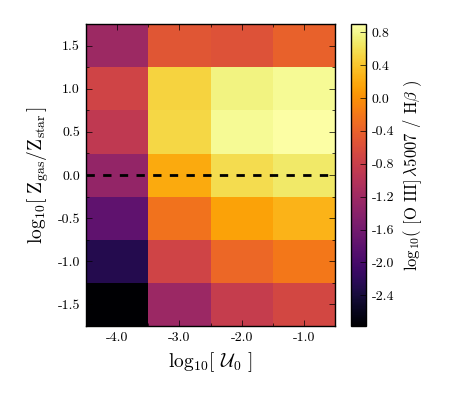
\includegraphics[width=0.283\linewidth]{figs/f27c.png}
    \caption{Impact of varying the gas phase metallicity (Z$_{\mathrm{gas}}$) for a fixed stellar metallicity (Z$_{\mathrm{star}}$; \logZeq{-1}). \emph{Left:} The standard BPT diagram. The blue lines show a standard model grid varying in ionization parameter and metallicity, where Z$_{\mathrm{gas}}$ = Z$_{\mathrm{star}}$. The markers show the models where Z$_{\mathrm{gas}}$ is decoupled from Z$_{\mathrm{star}}$.  All model points assume the same ionizing spectrum: a stellar population with constant SFR over 10\Myr and $\log_{10} \mathrm{Z}_{\mathrm{star}}/\mathrm{Z}_{\odot} = -1$. The color of the markers represent models with different ionization parameters. The circular marker shows the location where the gas phase metallicity equals the stellar metallicity, Z$_{\mathrm{gas}}=$Z$_{\mathrm{star}}$. The star-shaped marker shows the ``enriched model'' (\logZeq{-0.5}; Z$_{\mathrm{gas}}=3\,$Z$_{\mathrm{star}}$). \emph{Center \& Right:} The \nii/\ha (\emph{center}) and \oiii/\hb (\emph{right}) line ratios as a function of Z$_{\mathrm{gas}}$ and ionization parameter. The dashed line indicates where $\mathrm{Z}_{\mathrm{gas}}=\mathrm{Z}_{\mathrm{star}}$. Both line ratios increase as the gas metallicity is enhanced.}
    \label{fig:diffZ}
  \end{center}
\end{figure*}
%-------------------------------------------------------

We show the models with decoupled gas and stellar metallicities in Fig.~\ref{fig:diffZ}. These decoupled models reflect responses to gas inflow or localized enrichment with the same abundance pattern, or alternatively, can reflect abundance differences between the gas and stars in part due to the different elements that dominate the ISM cooling and emission lines and the stellar atmosphere.

For a fixed ionizing spectrum, an enhanced gas phase metallicity shifts line ratios to larger \nii/\ha and \oiii/\hb ratios by ${\sim}1\,$dex at all ionization parameters. This shift occurs because the metal-poor ionizing spectrum is harder and provides more ionizing photons, while the gas enriched in N and O produces larger BPT line ratios. This shift would be consistent with observations of galaxies at high redshift, which show extreme BPT line ratios, particularly at high \oiii/\ha.  Decoupling the gas and stellar metallicities is thus an enticing explanation for the optical emission lines.

Unlike the optical, where \oiii is one of the strongest optical emission lines, the \ciii$\lambda\lambda$1907,9 doublet is the strongest UV emission line after Ly$\alpha$. In Fig.~\ref{fig:diffZCO} we show how \ciii$\lambda$1907 emission responds to a change in gas phase metallicity for a fixed stellar metallicity of \logZeq{-1}. \ciii$\lambda$1907 is very sensitive to ionization parameter and weak at high metallicities. In an enriched gas model (Z$_{\mathrm{gas}}$ $>$ Z$_{\mathrm{star}}$) we would expect \ciii$\lambda$1907 to be weaker and the ratio of \oiii$\lambda$1666/\ciii$\lambda$1907 to be weaker. This is in conflict with observations, which show strong \ciii$\lambda$1907 emission and strong \oiii$\lambda$1666/\ciii$\lambda$1907 ratios, implying gas phase oxygen abundances at or below $12+\log_{10}(\mathrm{O}/\mathrm{H})\sim 8$. Thus, it is difficult to explaining the presence of both extreme \oiii/\ha ratios and strong \ciii emission in objects at high redshift without invoking a more peculiar abundance perscription that includes $\alpha$-enhancement and elevated N/O or C/O abundances. 

%-------------------------------------------------------
% diffZ CIII
%-------------------------------------------------------
\begin{figure*}
  \begin{center}
    \plottwo{figs/f28a.png}{figs/f28b.png}
    \caption{Changes in the \oiii/\ciii ratio from varying the gas phase abundances (Z$_{\mathrm{gas}}$) at fixed stellar metallicity (Z$_{\mathrm{star}}$; \logZeq{-1}). The dashed line indicates where the stellar and gas phase metallicities are equal. Unlike the BPT line ratios shown in Fig.~\ref{fig:diffZ}, which increase as $\mathrm{Z}_{\mathrm{gas}}$ gets larger than $\mathrm{Z}_{\mathrm{star}}$, the \oiii/\ciii ratio is largest when $\mathrm{Z}_{\mathrm{gas}}\lesssim \mathrm{Z}_{\mathrm{star}}$.}
    \label{fig:diffZCO}
  \end{center}
\end{figure*}
%-------------------------------------------------------

\subsubsection{Emission line equivalent widths} \label{sec:obs:UV:EWs}

Emission line equivalent widths (EWs) are frequently reported instead of fluxes. However, EWs are sensitive to the luminosity of the underlying continuum relative to the strength of the emission line.

To measure emission line equivalent widths from our models, we follow the methodology applied to observed data. In broad terms, the process involves subtracting the best-fit stellar continuum, and then fitting the residual emission line with a Gaussian. We generate two spectra with \FSPS, one that includes nebular emission lines and one that does not. We use the ``non-emission'' spectrum as the best-fit stellar continuum. \FSPS returns $\mathcal{F}_{\lambda}$ in \Lsun/\ang, which we convert to cgs units (erg/s/cm$^{-2}$/\ang) by assuming a total stellar mass of $M=10^7$\Msun\footnote{We chose this mass to match the observed properties of the \citet{Berg+2016} sample. However, we note that the \ciii equivalent widths presented here are not sensitive to that choice, since both the underlying UV stellar continuum and the \ciii luminosity scale directly with the flux of the same massive star population.} and a distance of 10$\,$Mpc. We subtract the continuum spectrum from the emission spectrum and fit the resultant scaled emission-line-only spectrum with \texttt{scipy.optimize.curvefit} \citep{SciPy} using a 3-parameter Gaussian function of the form:
\begin{equation}
    f(x) = a \cdot \exp \left( \frac{-(x-b)^2}{2c} \right),
\end{equation}
such that the integrated flux in the Gaussian is simply $\sqrt{2\pi} \cdot ac$ and an equivalent width with units of \ang. 

In Fig.~\ref{fig:CIIIew} we plot the model equivalent width of \ciii$\lambda\,1907,1909$ as a function of metallicity for a 1\Myr instantaneous burst, where we have added the equivalent widths of the \ciii$\lambda\,$1907 and \ciii$\lambda\,$1909.

The equivalent width of \ciii depends strongly on ionization parameter, where models with high ionization parameters produce larger \ciii equivalent widths. The equivalent widths are also strongly dependent on metallicity. The largest \ciii equivalent width (nearly 40\ang) is seen  at $\log_{10}(\mathrm{O}/\mathrm{H})\sim 8$, and declines toward both higher and lower metallicities. \ciii equivalent widths decrease much more rapidly towards high metallicities, and are essentially non-existent at solar and super-solar metallicities. \ciii equivalent widths decline to $\sim10$\ang at \logZeq{-2} due to the increasing deficit of carbon.

We compare the models in Fig.~\ref{fig:CIIIew} to measured equivalent widths and metallicities from the \citet{Berg+2016} and \citet{Senchyna+2017} samples, both of which also measure equivalent widths using single gaussian fits to the emission line. Fig.~\ref{fig:CIIIew} also includes the literature measurements compiled by \citet{Senchyna+2017}, which include nearby galaxies from \citet{Giavalisco+1996} (``G96'') and \citet{Leitherer+2011} (``L11'').

The models in Fig.~\ref{fig:CIIIew} are able to reproduce the range of observed \ciii equivalent widths and their distribution with metallicity. In particular, our models show weak \ciii equivalent widths at high metallicity ($\log_{10}(\mathrm{O}/\mathrm{H} \gtrsim 8.4$) and show the strongest \ciii equivalent widths at low metallicity ($\log_{10}(\mathrm{O}/\mathrm{H}){\sim} 8$). This behavior is in agreement with \citet{Senchyna+2017}, who suggested that there seemed to be a metallicity threshold in the observations, where large \ciii equivalent widths were only observed in galaxies with metallicities below $\log_{10}(\mathrm{O}/\mathrm{H})\sim 8.4$. Our model envelope naturally suppresses the \ciii EW at high metallicity, though perhaps not as strongly as is seen in the data.

%For galaxies with metallicities typical of present-day star forming galaxies, large \ciii equivalent widths require extreme ionization parameters (\logUeq{-1}). \ciii emission is strongest at $\log_{10}(\mathrm{O}/\mathrm{H})\sim 8$, where equivalent widths are comparable to that observed in the reionization era \citep{Stark+2015, Stark+2017}. As the gas phase metallicity continues to decrease, the \ciii equivalent widths eventually turn over to smaller values again. At the lowest metallicities in our model, we do not predict equivalent widths larger than 10-15\ang. This is likely due to the lack of available C in the gas (though see \S\ref{sec:gasZ} for a discussion variations in gas phase abundances).

%-------------------------------------------------------
% CIII equivalent widths
%-------------------------------------------------------
\begin{figure}
  \begin{center}
    \plotone{figs/f17.png}
    \caption{The equivalent width of \ciii$\lambda\,1907,1907$ as a function of metallicity for a 1\Myr instantaneous burst with $M=10^7$\Msun. The blue lines connect models of constant ionization parameter. \logUeq{-1} is shown in dark blue and \logUeq{-4} is shown in light blue. Models of constant metallicity are connected by the colored lines, from \logZeq{-1} in purple and \logZeq{0.0} in yellow. As noted in \citet{Senchyna+2017}, there seems to be a metallicity ceiling around $\log_{10}(\mathrm{O}/\mathrm{H})\sim 8$, above which \ciii emission is very weak. }
    \label{fig:CIIIew}
  \end{center}
\end{figure}
%-------------------------------------------------------

Higher ionization parameters produce larger \ciii equivalent widths at all metallicities. Thus, observations with large \ciii equivalent widths should be also biased toward high ionization parameters, and should have emission line ratios that similarly reflect that bias. We test this hypothesis in Fig.~\ref{fig:CIIIBPT}, where we show our models on optical diagnostic diagrams color-coded by their UV \ciii equivalent width. The left and middle panels show the BPT diagram and the O$_{32}$-R$_{23}$ diagram respectively. Models with large \ciii equivalent widths (redder colors) occupy the region of the BPT diagram with large values of \oiii/\hb and large ionization parameters. Similarly, the models with large \ciii equivalent widths have large O$_{32}$ ratios, also indicating high ionization parameters.

Finally, the right panel of Fig.~\ref{fig:CIIIBPT} shows the \ciii equivalent width as a function of the optical \oiii$\lambda\,5007$ equivalent width. Objects with large \oiii equivalent widths have been suggested as a means of optically selecting galaxies with strong UV \ciii emission \citep{Berg+2016, Senchyna+2017}. Our models confirm this correlation, although with an offset, due to the different metallicity dependence of carbon and oxygen line strength. The largest \ciii equivalent widths in the models do not coincide with the largest \oiii equivalent widths, since oxygen emission lines are strongest at a slightly higher metallicity ($\log_{10}(\mathrm{O}/\mathrm{H})\sim 8.4$) than the metallicity with peak \ciii emission ($\log_{10}(\mathrm{O}/\mathrm{H})\sim 8$). 

%-------------------------------------------------------
% CIII equivalent widths
%-------------------------------------------------------
\begin{figure*}
  \begin{center}
    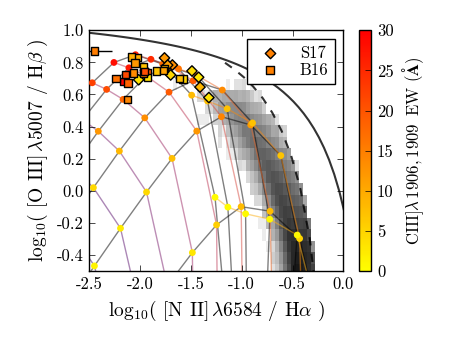
\includegraphics[width=0.283\linewidth]{figs/f18a.png}
    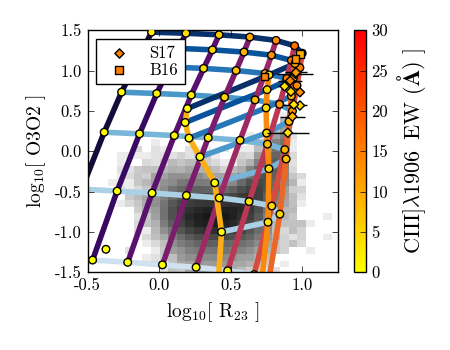
\includegraphics[width=0.283\linewidth]{figs/f18b.png}
    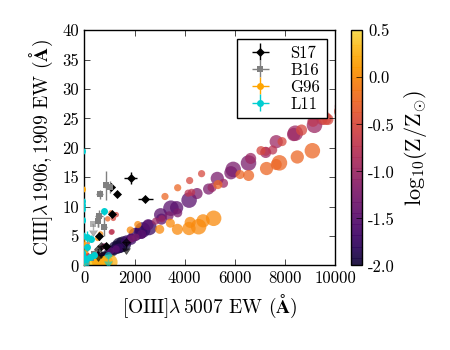
\includegraphics[width=0.283\linewidth]{figs/f18c.png}
    \caption{\emph{Left and Center:} Optical diagnostic diagrams color-coded by the equivalent width of \ciii$\lambda\,1907,1907$. Large \ciii equivalent widths occur in models with high ionization parameter, and thus coincide with observations that have large values of \oiii/\hb (\emph{left}) and large values of O3O2 (\emph{center}).  \emph{Right:} \ciii$\lambda\,1907,1907$ equivalent width as a function of \oiii$\lambda\,5007$ equivalent width. Large \ciii equivalent widths correlate with large \oiii equivalent widths.}
    \label{fig:CIIIBPT}
  \end{center}
\end{figure*}
%-------------------------------------------------------


%\begin{rotatetable*}
\begin{deluxetable*}{lccccccccccc}
\tabletypesize{\footnotesize}
%\tablewidth{0pt}
\tablecolumns{12}
\tablecaption{UV line fluxes given by the \CloudyFSPS models, assuming a 10\Myr CSFR at solar metallicity. The lines are given as $\log_{10}[\, \mathrm{F}_{\mathrm{line}} / \mathrm{F}_{\mathrm{H}\beta} \,]$.}
\tablehead{
\colhead{$\log_{10}\mathcal{U}_0$} &
\colhead{CIV} &
\colhead{CIV} &
\colhead{HeII} &
\colhead{OIII} &
\colhead{OIII} &
\colhead{AlII} &
\colhead{NIII} &
\colhead{SiIII} &
\colhead{SiIII} &
\colhead{CIII} &
\colhead{CIII}\\
\hline
\nocolhead{} &
\colhead{1548\ang} &
\colhead{1551\ang} &
\colhead{1640\ang} &
\colhead{1661\ang} &
\colhead{1666\ang} &
\colhead{1671\ang} &
\colhead{1752\ang} &
\colhead{1883\ang} &
\colhead{1892\ang} &
\colhead{1907\ang} &
\colhead{1909\ang}
}
\startdata
-4.0 & -5.3259 & -5.6272 & -2.6206 & -4.5499 & -4.1581 & -2.6228 & -4.7133 & -2.9867 & -3.2134 & -1.7065 & -1.8902 \\
-3.5 & -3.7689 & -4.0643 & -2.4183 & -3.7273 & -3.3355 & -2.5325 & -3.9159 & -2.6059 & -2.8317 & -1.3893 & -1.5728 \\
-3.0 & -2.6854 & -2.8647 & -2.3427 & -3.2949 & -2.9033 & -2.4825 & -3.5258 & -2.4548 & -2.6774 & -1.2797 & -1.4632 \\
-2.5 & -2.4156 & -2.4729 & -2.3021 & -3.1025 & -2.7121 & -2.4571 & -3.3794 & -2.4187 & -2.6303 & -1.2749 & -1.4583 \\
-2.0 & -2.3026 & -2.3483 & -2.2641 & -2.9781 & -2.5905 & -2.4446 & -3.2914 & -2.4054 & -2.5935 & -1.2792 & -1.4624 \\
-1.5 & -2.1895 & -2.2539 & -2.2261 & -2.8917 & -2.5093 & -2.4448 & -3.2333 & -2.3956 & -2.5561 & -1.2736 & -1.4564 \\
-1.0 & -2.0432 & -2.1298 & -2.1901 & -2.8149 & -2.4401 & -2.4382 & -3.1827 & -2.3826 & -2.5224 & -1.2555 & -1.4377 \\
\enddata
\tablecomments{Only a portion of this table is shown here to demonstrate its form and content. A machine-readable version of the full table is available online.}
\label{tab:lineStrengths}
\end{deluxetable*}
%\end{rotatetable*}